\documentclass[aspectratio=169]{beamer}

% ---------- Theme & Farben ----------
\usetheme{Madrid}
\usecolortheme{whale}
\setbeamerfont{frametitle}{size=\large, series=\bfseries}
\setbeamertemplate{navigation symbols}{}
\setbeamertemplate{footline}[frame number]

\usepackage[ngerman]{babel}
\usepackage{amsmath, amssymb}
\usepackage{booktabs}
\usepackage{multirow}
\usepackage{graphicx}
\usepackage{xcolor}
\usepackage{colortbl}

\graphicspath{{./}}

\definecolor{bestgreen}{RGB}{0,140,0}
\definecolor{warnred}{RGB}{200,40,40}

% ---------- Meta-Informationen ----------
\title[Neuronale Operatoren]{Neuronale Operatoren zur\\
       Strömungssimulation um Kristalle}
\subtitle{U-Net vs.\ Fourier Neural Operator -- Aktueller Stand}
\author{Paul Baselt}
\date{\today}
\institute{Betreuer-Meeting -- Masterarbeit}

% =============================================================================
\begin{document}
% =============================================================================

\begin{frame}
  \titlepage
\end{frame}

\begin{frame}{Agenda}
  \tableofcontents
\end{frame}

% =============================================================================
\section{Grundlagen \& Problemstellung}
% =============================================================================

% --- Folie 1/2: Physikalische Situation ---
\begin{frame}{Physikalische Situation \& Lernziel}
  \begin{columns}[T]
    \column{0.56\textwidth}
      \textbf{Setup:}
      \begin{itemize}
        \item Kristalle eingebettet in viskose Matrix
        \item Gebiet: $256\times256$-Gitter, $[-1,1]^2$\,km
        \item Stokes-Gleichungen (niedrige Reynolds-Zahl):
          \[
            -\nabla p + \eta\,\Delta\mathbf{v} = 0, \qquad \nabla\cdot\mathbf{v}=0
          \]
        \item Numerische Referenz: \textbf{LaMEM} (FEM-Solver) -- korrekt, aber rechenintensiv
      \end{itemize}
      \vspace{8pt}
      \textbf{Ziel:} Neuronales Netz sagt Strömungsfeld vorher -- \emph{ohne} FEM-Simulation.

    \column{0.40\textwidth}
      \begin{block}{Eingabe $\to$ Ausgabe}
        \textbf{4 Eingangskanäle:}
        \begin{itemize}
          \item Kristallmaske (Typ)
          \item Normalisierte x- und z Koordinaten 
          \item Signed Distance Field (SDF)
        \end{itemize}
        \vspace{6pt}
        \textbf{Ausgabe (Lernziel):}\\[4pt]
        $\hat\psi \in \mathbb{R}^{256\times256}$
        \vspace{6pt}

        \textbf{Abgeleitet (Nachschritt):}\\[4pt]
        $\hat{\mathbf{v}} = \operatorname{curl}(\hat\psi)$
      \end{block}
  \end{columns}
\end{frame}

% --- Folie 2/2: Warum Stromfunktion ---
\begin{frame}{Warum Stromfunktion $\psi$?}
  \begin{columns}[T]
    \column{0.54\textwidth}
      \textbf{Definition der Stromfunktion:}
      \[
        v_x = \frac{\partial\psi}{\partial z}, \qquad v_z = -\frac{\partial\psi}{\partial x}
      \]

      \vspace{6pt}
      \textbf{Inkompressibilität automatisch erfüllt:}
      \begin{align*}
        \nabla\cdot\mathbf{v}
          &= \frac{\partial v_x}{\partial x} + \frac{\partial v_z}{\partial z}
           = \frac{\partial^2\psi}{\partial x\partial z}
           - \frac{\partial^2\psi}{\partial z\partial x}
           = 0
      \end{align*}
      \small(Satz von Schwarz: gemischte partielle Ableitungen kommutieren)
      \normalsize
      \vspace{4pt}

      Das Netz lernt \emph{nur} $\hat\psi$ -- Inkompressibilität
      ist \textbf{strukturell} garantiert.

    \column{0.42\textwidth}
      \begin{block}{Vorteile}
        \begin{itemize}
          \item Kein Divergenz-Strafterm nötig
          \item Lernproblem: 2 Felder $\to$ 1 Skalar
          \item Fehleranalyse einfacher
        \end{itemize}
      \end{block}

      \vspace{6pt}
      \begin{alertblock}{Konsequenz}
        $\varepsilon_v$ ist \emph{immer} größer als
        $\varepsilon_\psi$: Ableitung (Nachschritt)
        verstärkt hochfrequente Fehler.
      \end{alertblock}
  \end{columns}
\end{frame}

% --- Folie 3: Verlustfunktionen ---
\begin{frame}{Verlustfunktionen}
  \begin{columns}[T]
    \column{0.56\textwidth}
      \begin{block}{FNO -- Composite-Loss}
        \[
          \mathcal{L} =
            \underbrace{\|\hat\psi - \psi\|_2^2}_{\text{MSE}}
          + \alpha\underbrace{\|\nabla\hat\psi - \nabla\psi\|_2^2}_{\text{Gradient-Term}}
          + \beta\underbrace{\|\hat\psi\big|_{\partial\Omega}\|_2^2}_{\text{Rand-Term}}
        \]
        \begin{itemize}
          \item $\alpha$: Warmup über 5 Epochen, Zielwert~$0.1$
          \item $\beta = 0.01$\quad (Dirichlet: $\psi = 0$ am Rand)
          \item Gradient-Term erzwingt korrekte Ableitungen
          \item Rand-Term stellt $\hat\psi\big|_{\partial\Omega} = 0$ sicher
        \end{itemize}
      \end{block}

    \column{0.40\textwidth}
      \begin{block}{U-Net -- Loss}
        \[
          \mathcal{L} = \|\hat\psi - \psi\|_2^2
        \]
        Nur MSE -- kein Gradient- oder Rand-Term.\\[6pt]
        Das Netz lernt implizit die Randwerte aus den Trainingsdaten.
      \end{block}

      \vspace{8pt}
      \begin{block}{Optimizer}
        \begin{tabular}{ll}
         Adam für beide
        \end{tabular}
      \end{block}
  \end{columns}
\end{frame}

% --- Folie 4: Evaluationsmetriken ---
\begin{frame}{Evaluationsmetriken \& Best-Checkpoint-Strategie}
  \begin{columns}[T]
    \column{0.48\textwidth}
      \textbf{Evaluationsmetriken:}
      \vspace{6pt}
      \renewcommand{\arraystretch}{1.4}
      \begin{tabular}{ll}
        \toprule
        Metrik & Bedeutung \\
        \midrule
        $\varepsilon_\psi^{\text{rel}}$ & Mittl.\ rel.\ L2 in $\psi$ \\
                                        & \emph{Hauptmetrik} \\[2pt]
        $\varepsilon_v^{\text{rel}}$    & Mittl.\ rel.\ L2 in $|\mathbf{v}|$ \\[2pt]
        $\varepsilon_\psi^{\max}$       & Maximaler Fehler in $\psi$ \\[2pt]
        div\,rms                        & RMS-Divergenz ($\to 0$) \\
        \bottomrule
      \end{tabular}

    \column{0.48\textwidth}
      \begin{block}{Best-Checkpoint-Strategie}
        Auswertung \textbf{nicht} am letzten Epoch,
        sondern am Epoch mit dem besten Validierungs-Loss.\\[8pt]
        \textbf{Warum wichtig?}
        \begin{itemize}
          \item Modell kann nach dem besten Punkt wieder schlechter werden
          \item Ohne LR-Scheduler: Oszillationen um Minimum möglich
        \end{itemize}
      \end{block}
  \end{columns}
\end{frame}

% --- Folie 5a: Datengenerierung ---
\begin{frame}{Datengenerierung \& Experiment-Übersicht}
  \begin{columns}[T]
    \column{0.44\textwidth}
      \textbf{Datensätze (LaMEM-FEM):}
      \begin{itemize}
        \item Drei unabhängige Seeds:\\
              Training / Validierung / Test
        \item Training 1000 Samples pro Kristallzahl $n$
        \item Validierung 100 Samples pro Kristallzahl $n$
        \item Training 10 Samples pro Kristallzahl $n$
      \end{itemize}

    \column{0.52\textwidth}
      \renewcommand{\arraystretch}{1.45}
      \begin{tabular}{cllll}
        \toprule
        Exp & Training & Test & OOD \\
        \midrule
        1 & $n=1$          & $n=1$          & --             \\
        2 & $n=1\ldots10$  & $n=1\ldots10$  & $n=11\ldots25$ \\
        3 & $n=1\ldots25$  & $n=1\ldots25$  & $n=26\ldots84$ \\
        \bottomrule
      \end{tabular}
  \end{columns}

  \vspace{16pt}
  \begin{itemize}
    \item \textbf{Exp.~1}: Hyperparameter-Suche (lr, batch) -- ein Kristall
    \item \textbf{Exp.~2}: Multi-Kristall-Generalisierung, OOD bis $n=25$
    \item \textbf{Exp.~3}: Stress-Test mit extremem OOD bis $n=84$
  \end{itemize}
\end{frame}

% --- Folie 5b: Trainingssetup ---
\begin{frame}{Trainingssetup \& Hyperparameter}
  \begin{columns}[T]
    \column{0.50\textwidth}
      \renewcommand{\arraystretch}{1.4}
      \begin{tabular}{lll}
        \toprule
        Parameter & U-Net & FNO \\
        \midrule
        Batch-Größe     & 8 / 16  & 8 / 16 \\
        Epochen (Exp.~1) & 180    & 100 \\
        Optimizer       & Adam    & Adam + Clip \\
        Loss            & Composite* & Composite* \\
        \bottomrule
      \end{tabular}
      \vspace{6pt}

      \small
      ${}^*$Composite: MSE + Gradient-Term + Rand-Term\\

    \column{0.46\textwidth}
      \textbf{Lernraten} (beide Modelle):
      \vspace{6pt}

      \renewcommand{\arraystretch}{1.4}
      \begin{tabular}{cc}
        \toprule
        $10^{-4}$ & $5\cdot10^{-4}$ \\
        $10^{-3}$ & $5\cdot10^{-3}$ \\
        \bottomrule
      \end{tabular}
      \vspace{10pt}

      \textbf{Checkpoint-Strategie:}\\
      Bestes Modell nach Val-Loss wird gespeichert
      (nicht zwingend das letzte Epoch).
  \end{columns}
\end{frame}

% =============================================================================
\section{Modellarchitekturen}
% =============================================================================

\begin{frame}{Modellarchitekturen: U-Net vs.\ FNO}
  \begin{columns}[T]
    \column{0.47\textwidth}
      \begin{block}{U-Net (CNN-basiert)}
        \begin{itemize}
          \item Encoder--Decoder mit Skip-Connections
          \item Faltungen: lokaler $k\times k$-Ausschnitt
          \item \textcolor{bestgreen}{Stärke:} scharfe Kanten,\\
                Kristallkontur
          \item \textcolor{warnred}{Schwäche:} globale\\
                Strömungsstruktur
          \item 32 Basiskanäle, 4 Encoder-Ebenen
        \end{itemize}
      \end{block}

    \column{0.47\textwidth}
      \begin{block}{FNO (Fourier Neural Operator)}
        \begin{itemize}
          \item Operiert direkt im Fourier-Raum
          \item FFT~$\to$ Modengewichtung~$\to$~IFFT\\
                + lokaler linearer Bypass
          \item \textcolor{bestgreen}{Stärke:} globale Spektral-Features,\\
                $\mathcal{O}(N\log N)$
          \item Gitterunabhängig (theoretisch)
          \item Natürlich für glatte Stokes-Felder
          \item Width\,=\,64, Depth\,=\,4, Modes\,=\,16
        \end{itemize}
      \end{block}
  \end{columns}

  \vspace{10pt}
  \begin{center}
    Beide Modelle: Eingabe $256\times256\times4$, Ausgabe $256\times256\times1$~($\hat\psi$).\\
    \small Geschwindigkeitsfeld $\hat{\mathbf{v}} = \operatorname{curl}(\hat\psi)$ als Nachschritt -- kein eigenes Lernziel.
  \end{center}
\end{frame}

% =============================================================================
\section{Experiment~1: Einzelkristall ($n=1$)}
% =============================================================================
% Ab hier muss ich das händisch ergänzen und Auswertung für meine Ergebnisse
% --- Hyperparameter FNO ---
\begin{frame}{Exp~1 -- FNO Hyperparameter-Suche (100~Epochen)}
  \begin{columns}[T]
    \column{0.50\textwidth}
      \textbf{Batch-Größe 8:}
      \vspace{4pt}
      \renewcommand{\arraystretch}{1.35}
      \begin{tabular}{crrl}
        \toprule
        Lernrate & $\varepsilon_\psi^{\text{rel}}$ & $\varepsilon_v^{\text{rel}}$ & \\
        \midrule
        $5\!\times\!10^{-4}$ & 2.61\,\% & 3.82\,\% \\
        $5\!\times\!10^{-3}$ & \textcolor{bestgreen}{\textbf{2.07\,\%}} & 4.13\,\% & $\leftarrow$ best\\
        $10^{-3}$            & 4.18\,\% & 4.89\,\% & \\
        $10^{-4}$            & 5.85\,\% & 10.56\,\% & \\
        \bottomrule
      \end{tabular}

    \column{0.46\textwidth}
      \textbf{Batch-Größe 16:}
      \vspace{4pt}
      \renewcommand{\arraystretch}{1.35}
      \begin{tabular}{crrl}
        \toprule
        Lernrate & $\varepsilon_\psi^{\text{rel}}$ & $\varepsilon_v^{\text{rel}}$ & \\
        \midrule
        $5\!\times\!10^{-4}$ & \textcolor{bestgreen}{\textbf{1.62\,\%}} & 3.44\,\% & $\leftarrow$ best \\
        $10^{-4}$            & 5.10\,\% & 8.18\,\% & \\
        $10^{-3}$            & 2.06\,\% & 3.02\,\% & \\
        $5\!\times\!10^{-3}$ & 2.31\,\% & 4.15\,\% & \\      
        \bottomrule
      \end{tabular}
  \end{columns}

  \vspace{10pt}
  \textbf{Beobachtungen:}
  \begin{itemize}
    \item Optimales Fenster: lr~$\in [5\!\times\!10^{-4},\,5\!\times\!10^{-3}]$
    \item Kleinere Batch-Größe hilft -- bs\,=\,8 verbessert bs\,=\,16 von 2.07\,\% auf 1.62\,\%
  \end{itemize}
\end{frame}

% --- Hyperparameter U-Net ---
\begin{frame}{Exp~1 -- U-Net Hyperparameter-Suche (180~Epochen, Best-Checkpoint)}
  \begin{columns}[T]
    \column{0.48\textwidth}
      \textbf{Batch-Größe 8:}
      \vspace{4pt}
      \renewcommand{\arraystretch}{1.35}
      \begin{tabular}{crrl}
        \toprule
        Lernrate & $\varepsilon_\psi^{\text{rel}}$ & $\varepsilon_v^{\text{rel}}$ & \\
        \midrule
        $10^{-3}$            & 6.0\,\% & 9.3\,\% \\
        $5\!\times\!10^{-3}$ & 5.5\,\% & 8.5\,\% & \\
        $5\!\times\!10^{-4}$ & 5.9\,\% & 9.6\,\% & \\
        $10^{-4}$            & 6.5\,\% & 12.7\,\% & \\
        \bottomrule
      \end{tabular}

    \column{0.48\textwidth}
      \textbf{Batch-Größe 16:}
      \vspace{4pt}
      \renewcommand{\arraystretch}{1.35}
      \begin{tabular}{crrl}
        \toprule
        Lernrate & $\varepsilon_\psi^{\text{rel}}$ & $\varepsilon_v^{\text{rel}}$ & \\
        \midrule
        $10^{-3}$            & 13.9\,\% & 22.1\,\% & \\
        $5\!\times\!10^{-4}$ & 15\,\% & 29.9\,\% & \\
        $10^{-4}$            & 13.5\,\%  & 23.1\,\% & \\
        $5\!\times\!10^{-3}$ & 24,\% & 53\,\% & \\
        \bottomrule
      \end{tabular}
  \end{columns}

  \vspace{10pt}
  \textbf{Beobachtungen:}
  \begin{itemize}
    \item \textbf{Batch\,8 deutlich besser als Batch\,16} -- $5.17\,\%$ vs.\ $8.56\,\%$
    \item Velocity-Fehler $\approx 3\times$ größer als $\psi$-Fehler (Ableitung als Nachschritt)
    \item Lernrate $10^{-3}$ optimal für bs\,=\,8; Variation hat mäßigen Einfluss
  \end{itemize}
\end{frame}

% --- Trainingskurven FNO---
\begin{frame}{Exp~1 -- Trainingskurven (jeweils bestes Modell)}
  \begin{columns}[c]
    \column{0.48\textwidth}
      \centering
      \textbf{FNO} \quad (bs\,=\,16, lr\,$=5\!\times\!10^{-4}$, 100~Ep.)\\[4pt]
      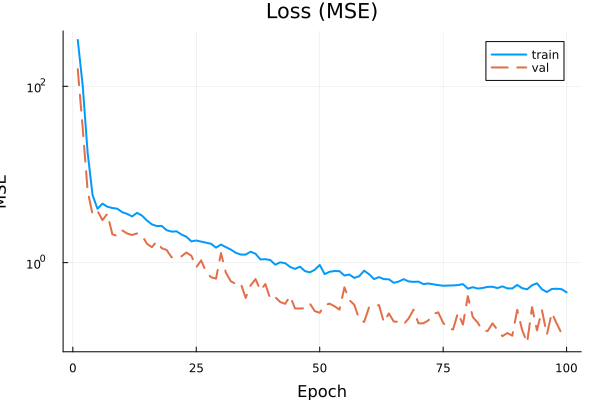
\includegraphics[width=\linewidth]{Bilder/FNO_16_Best.png}
      \small\\[2pt]
    \column{0.48\textwidth}
      \centering
      \textbf{FNO} \quad (bs\,=\,8, lr\,$=5\!\times\!10^{-3}$, 180~Ep.)\\[4pt]
      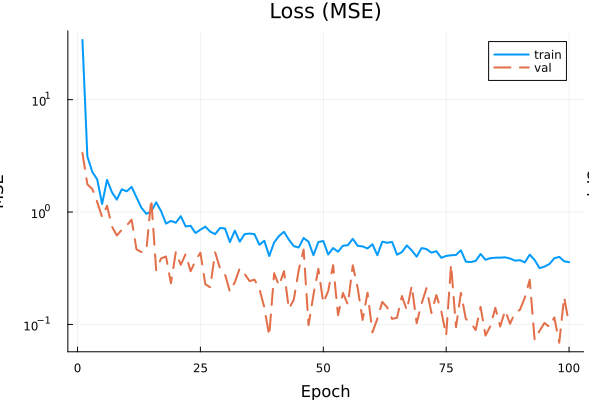
\includegraphics[width=\linewidth]{Bilder/FNO_8_Best.png}
      \small\\[2pt]
  \end{columns}
\end{frame}

% --- Qualitatives Ergebnis FNO psi ---
\begin{frame}{Exp~1 -- Qualitative Ergebnisse: Stromfunktion $\psi$}
      
\includegraphics[width=\linewidth]{Bilder/001_rel0.0261_psi.png}
      \vspace{1pt}
      
\includegraphics[width=\linewidth]{Bilder/002_rel0.0265_psi.png}
  \small
  \textit{Referenz (LaMEM) \;|\; Vorhersage \;|\; Absoluter Fehler~$\Delta\psi$}\\
  FNO-Fehler diffus und klein; U-Net zeigt leicht stärkere Abweichungen am Kristallrand.
\end{frame}

% --- Qualitatives Ergebnis FNO v ---
\begin{frame}{Exp~1 -- Qualitative Ergebnisse: Stromfunktion $\psi$}
      
\includegraphics[width=\linewidth]{Bilder/001_rel0.0261_vel.png}
      \vspace{1pt}
      
\includegraphics[width=\linewidth]{Bilder/002_rel0.0265_vel.png}
  \small
  \textit{Referenz (LaMEM) \;|\; Vorhersage \;|\; Absoluter Fehler~$\Delta v$}\\
  FNO-Fehler diffus und klein; U-Net zeigt leicht stärkere Abweichungen am Kristallrand.
\end{frame}

% --- Trainingskurven U-Net---
\begin{frame}{Exp~1 -- Trainingskurven (jeweils bestes Modell)}
      \textbf{U-Net} \quad (bs\,=\,8, lr\,$=5\!\times\!10^{-3}$, 180~Ep.)\\[4pt]
      \centering
      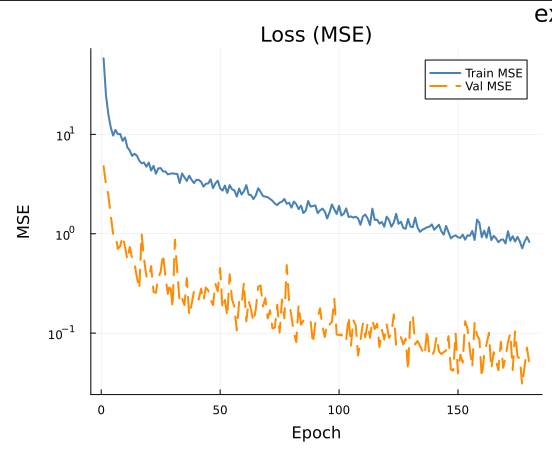
\includegraphics[width=0.5\textwidth]{Bilder/UNET_8_Best.png}
\end{frame}

% --- Qualitatives Ergebnis U-Net psi ---
\begin{frame}{Exp~1 -- Qualitative Ergebnisse: Stromfunktion $\psi$}
      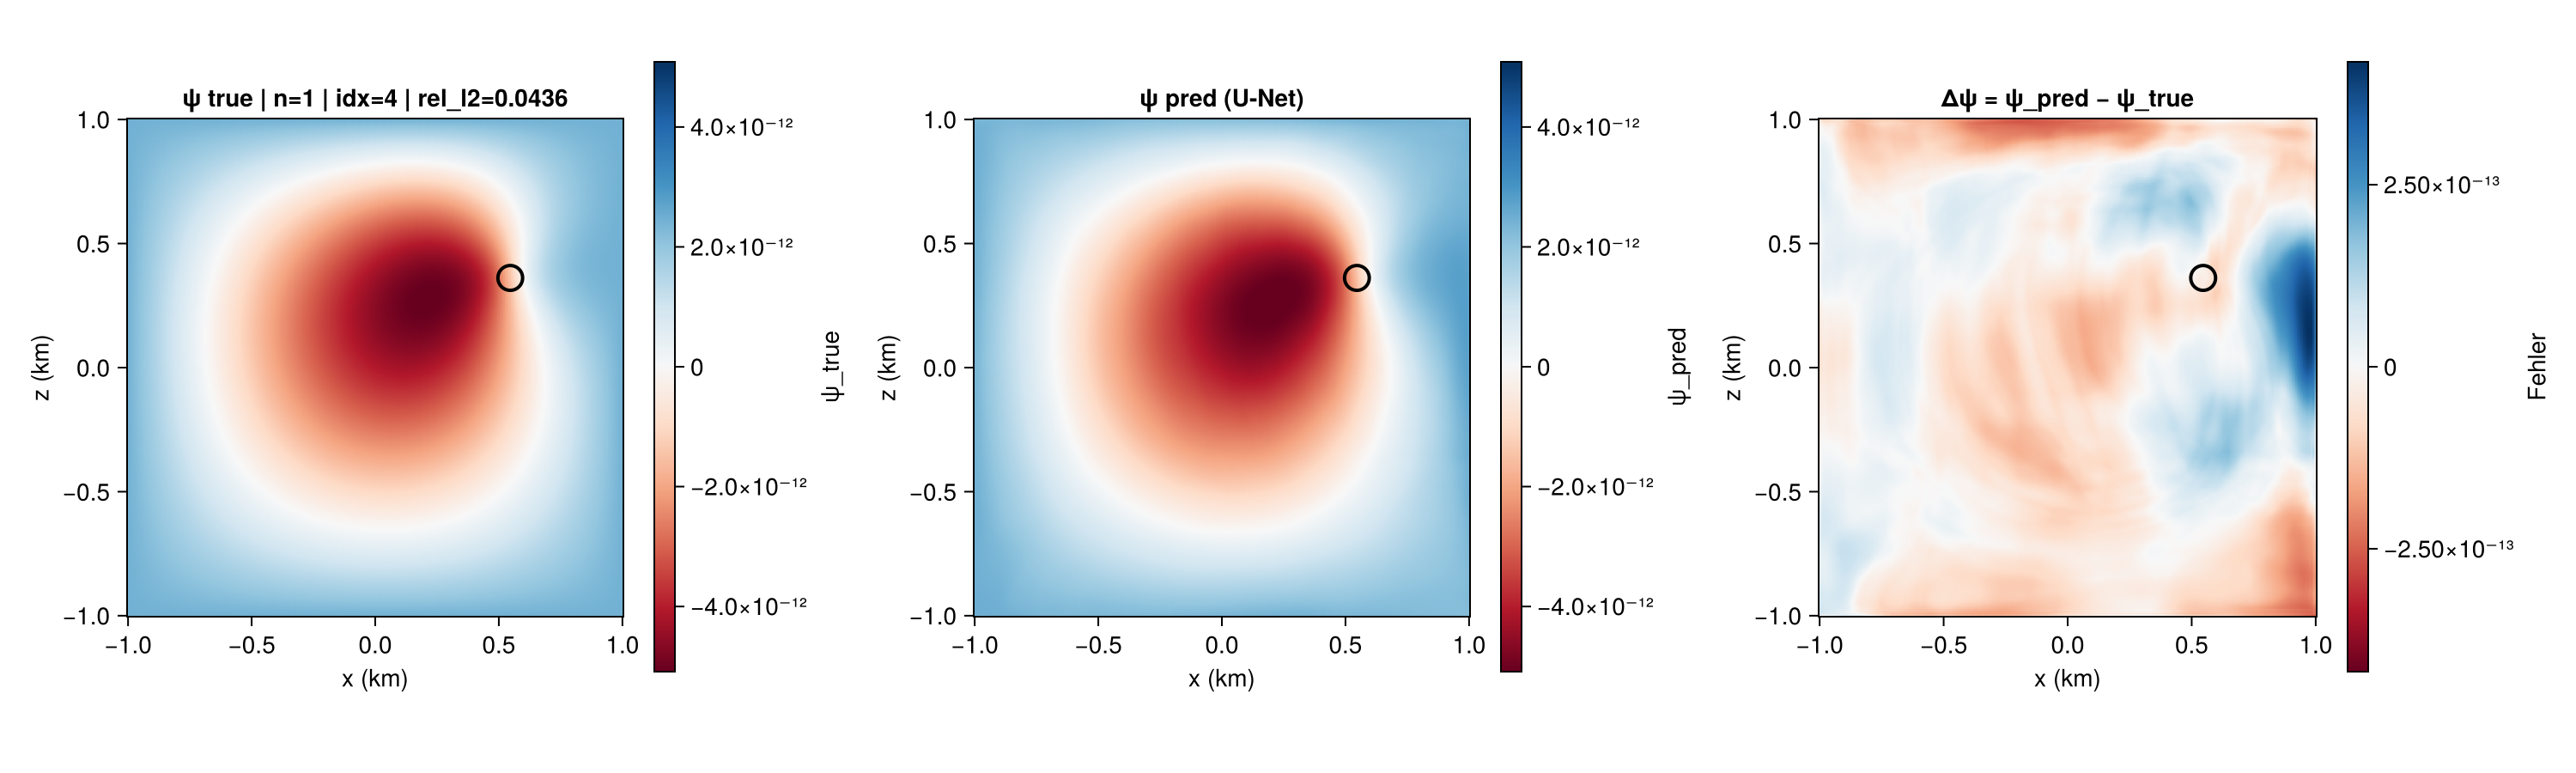
\includegraphics[width=\linewidth]{Bilder/sample_0004_rel0.0436_psi.png}
  \textit{Referenz (LaMEM) \;|\; Vorhersage \;|\; Absoluter Fehler~$\Delta\psi$}\\
  U-Net-Fehler diffus und klein; U-Net zeigt leicht stärkere Abweichungen am Kristallrand.
\end{frame}

% --- Qualitatives Ergebnis U-Net v ---
\begin{frame}{Exp~1 -- Qualitative Ergebnisse: Stromfunktion $\psi$}
      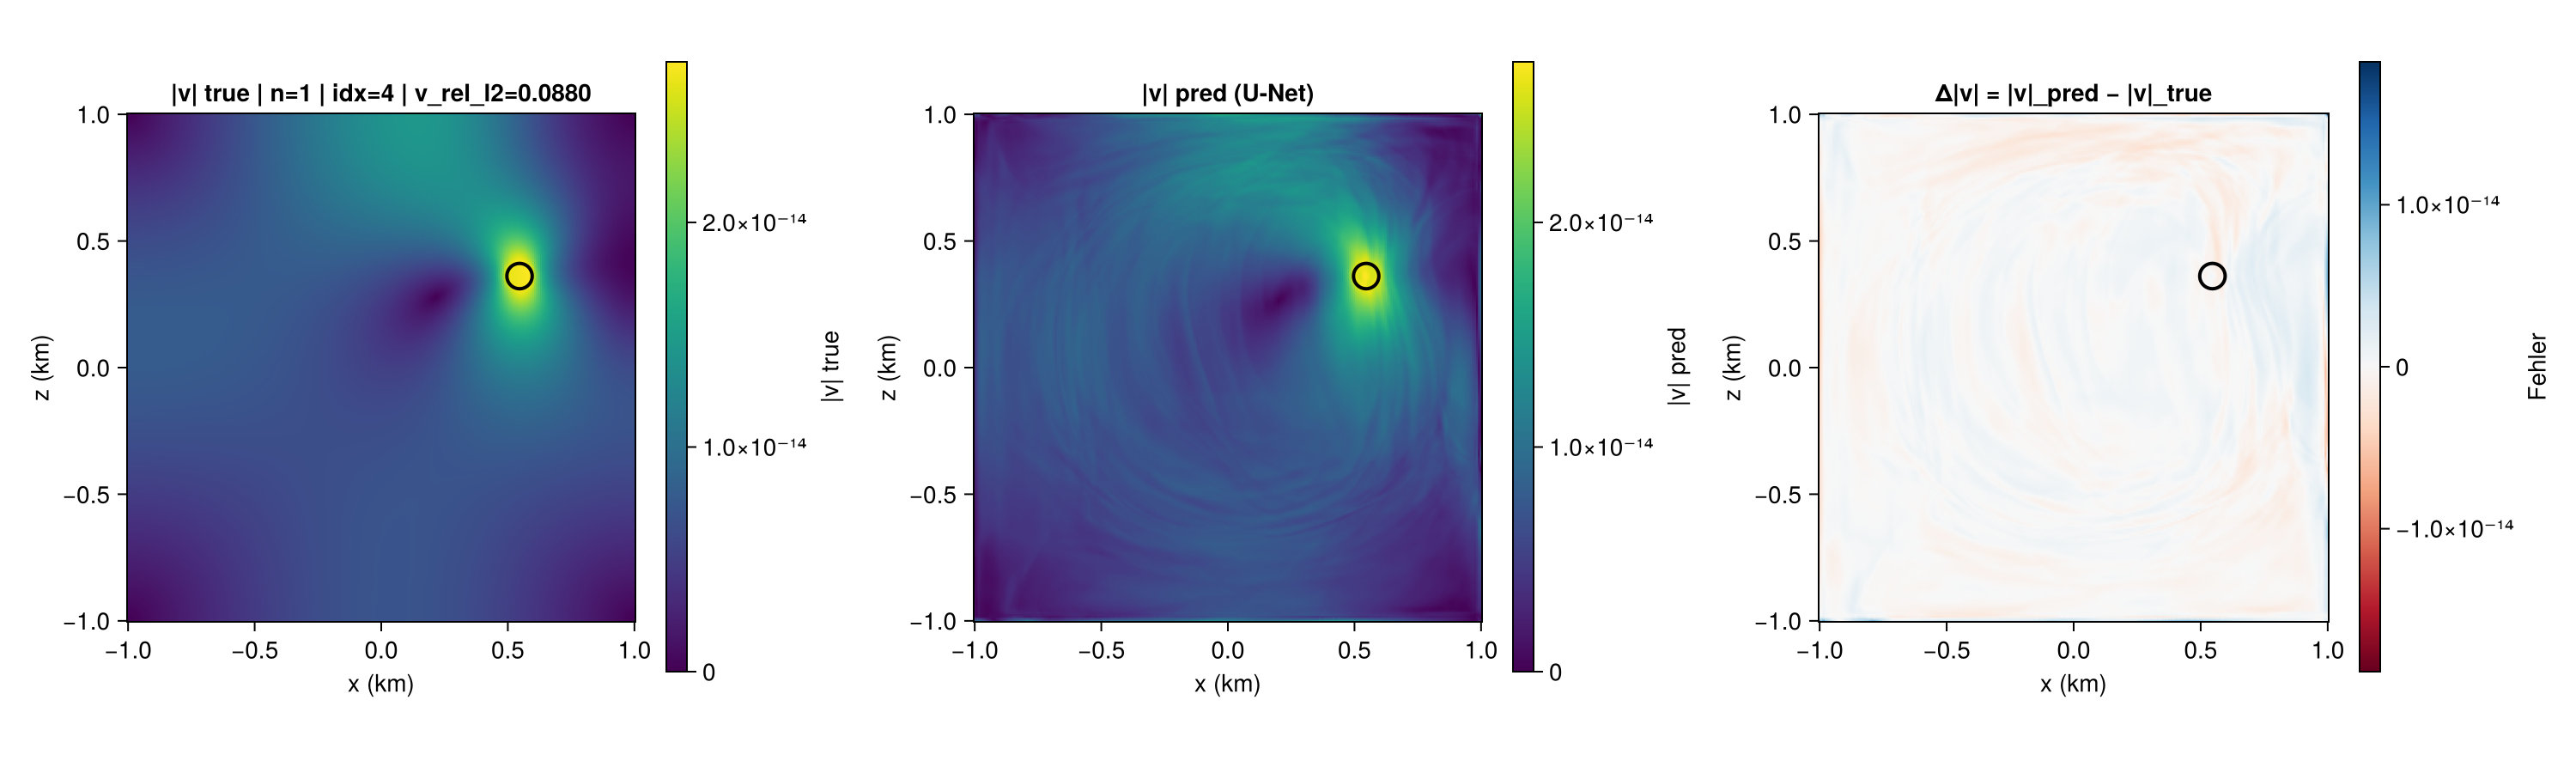
\includegraphics[width=\linewidth]{Bilder/sample_0004_rel0.0436_vel.png}
  \textit{Referenz (LaMEM) \;|\; Vorhersage \;|\; Absoluter Fehler~$\Delta v$}\\
  U-Net-Fehler diffus und klein; U-Net zeigt leicht stärkere Abweichungen am Kristallrand.
\end{frame}

% =============================================================================
\section{Analyse \& Diskussion}
% =============================================================================
% --- Gesamtvergleich ---
\begin{frame}{Gesamtvergleich: FNO vs.\ U-Net}
  \begin{center}
    \renewcommand{\arraystretch}{1.45}
    \begin{tabular}{llcc}
      \toprule
      Experiment & Modell & $\varepsilon_\psi^{\text{rel}}$ & $\varepsilon_v^{\text{rel}}$ \\
      \midrule
      \multirow{2}{*}{Exp-1 ($n=1$)}
        & \textbf{FNO} (bs\,=\,16, 100~Ep.)
          & \textcolor{bestgreen}{\textbf{1.62\,\%}} & \textcolor{bestgreen}{\textbf{3,44\,\%}} \\
        & U-Net (bs\,=\,8, 180~Ep.)
          & 5.5\,\% & 8.5\,\% \\
    \end{tabular}
  \end{center}
\end{frame}

% =============================================================================
\end{document}
% =============================================================================
